\chapter{Implementation}
\label{chapter:implementation}

This chapter focuses on the implementation of the components proposed in section \ref{sec:extended-design}. It describes how the backend functionalities, such as caching mechanisms, data acquisition workflows, and the \ac{SSVC} recommendation process, were realized to ensure efficient data handling and seamless integration with external systems. Additionally, the chapter explains how the frontend was implemented to support user interactions, including role-specific remediation-strategies and data visualization. This implementation bridges the gap between architectural design and a functional, scalable system.

\section{Backend Components}
\label{sec:backend-components}

This section explains the main backend building blocks, focusing on data storage, retrieval logic, and the mechanisms used to ensure up-to-date information.

\subsection{Caching Mechanism and Repository Layer}
\label{subsec:caching-repository}

A central piece of functionality is the storage of previously retrieved data. Two core strategies are employed to manage data retrieval: \textbf{Pre-Check} and \textbf{Scheduled Refresh}.

The \textbf{Pre-Check} strategy involves querying the internal repository whenever a vulnerability request arises. The system first checks whether a corresponding \textit{Vulnerability Data Entity} already exists. If it does, the existing record is returned. If no such entry is found, the system creates a new entity while simultaneously checking the local \ac{OSV} database for the associated \ac{CVSS} vector. If the vector is not available locally, an external \ac{API} call to the \ac{NVD} is performed to retrieve the missing details. In parallel, the \ac{EPSS} score is fetched from the external \texttt{first.org} \ac{API}, as it is not stored locally (see section~\ref{subsec:backend-responsibilities}).

The \textbf{Scheduled Refresh} strategy ensures data freshness through a nightly update cycle. This process starts 30 minutes after the \ac{OSV} database update (see section ~\ref{sec:current-design}), ensuring that the most recent vulnerability information is available. During this cycle, the system updates the entire dataset by performing batch requests for \ac{EPSS} scores via the \texttt{first.org} \ac{API} and individual requests to the \ac{NVD} for missing \ac{CVSS} details not available in the local \ac{OSV} database, as the \ac{NVD} does not support batch queries for \ac{CVE} IDs.\footnote{\url{https://nvd.nist.gov/developers/vulnerabilities}}

If either the \ac{CVSS} or \ac{EPSS} data cannot be retrieved, the system transitions to an \texttt{Error} state, returning a severity score of \textbf{10.1}. This value is highlighted in pink on the frontend to prompt user action (see section~\ref{subsec:handling-missing-data}).

\noindent
\paragraph{Example of a Caching Strategy (Pseudocode)}
\label{par:example-caching-strategy}

\begin{verbatim}
// Caching Strategy Pseudocode

// Check if vulnerability exists
if (existsInRepository(cveId)) {
    return getFromRepository(cveId);
}

// Create new entity and fetch data
entity = createNewEntity(cveId);
entity.cvssVector = getFromOsv(cveId) ?? fetchFromNvd(cveId);
entity.epssScore  = fetchFromFirstOrg(cveId);

// Save and return entity
saveToRepository(entity);
return entity;
\end{verbatim}

\noindent
If any data retrieval fails, the process is aborted, and the system proceeds as described in section~\ref{subsec:handling-missing-data}.

\subsection{Scheduled Refresh Mechanism}
\label{subsec:scheduled-refresh}

The \textbf{Scheduled Refresh} strategy ensures data freshness through a nightly update cycle. This process starts 30 minutes after the \ac{OSV} database update, ensuring that the most recent vulnerability information is available.

During this cycle, the system iterates through all existing \textit{Vulnerability Data Entities} and updates each entry as follows:
\begin{itemize}
    \item The local \ac{OSV} database is queried for the latest \ac{CVSS} vector.
    \item If the vector is not found locally, an external \ac{API} call is made to the \ac{NVD}.
    \item In parallel, the \ac{EPSS} scores are fetched in a batch from the external \texttt{first.org} \ac{API}, as it is not cached locally.
\end{itemize}

If any data retrieval fails, the system aborts the update for the affected entry and proceeds as described in section~\ref{subsec:handling-missing-data}. Successfully updated entities are saved back to the repository, ensuring the dataset remains accurate and current.

\noindent
\paragraph{Daily Vulnerability-Data Update (Pseudocode)}
\label{par:daily-vulnerability-update-short}

\begin{verbatim}
// Scheduled job: runs daily at 00:30
scheduleRecurringTask("vulnerability-data-update", "0 30 0 * * *") {
    updateVulnerabilityData();
}

function updateVulnerabilityData() {
    // Fetch all vulnerabilities
    entities = vulnerabilityDataRepository.findAll();

    // Batch-fetch EPSS scores
    epssScores = fetchBatchEpssScores(collectCveIds(entities));

    // Update each entity
    for each entity in entities {
        entity.epssScore  = epssScores.get(entity.cveId);
        [entity.cvssScore, entity.cvssVector] =
        fetchCvssScoreAndVector(
            entity.cveId,
            entity.vulnId
    );
        entity.severityScore = calculateSeverityScore(entity);
        entity.severityScoreLastUpdated = now();

        // Save updated entity
        vulnerabilityDataRepository.save(entity);
    }
}
\end{verbatim}

\paragraph{SSVC Recommendation Endpoint}
\label{par:ssvc-recommendation-endpoint}

The \ac{SSVC} recommendation endpoint, part of the controller layer, allows the frontend to submit tailored remediation plans. As described in section \ref{subsec:ssvc-process}, this endpoint integrates role-specific decisions into the backend’s controller layer. These recommendations are stored in the backend for integration with other vulnerability metrics. The pseudo-implementation is as follows:

\noindent
\paragraph{Updating SSVC Recommendation (Pseudocode)}
\label{par:update-ssvc-recommendation}

\begin{verbatim}
// For a POST request to "/api/.../vulnerabilities/{vulnId}/ssvc"
function updateSsvc(vulnId, ssvcRecommendation):
    // Retrieve the vulnerability record by its ID
    data = repository.findById(vulnId)
    
    // If found, update recommendation and save
    if data:
        data.ssvcRecommendation = ssvcRecommendation
        repository.save(data)
    
    // Return success response
    return HTTP_200_OK
\end{verbatim}

This process ensures that:
\begin{itemize}
  \item \ac{SSVC} recommendations are properly stored for each vulnerability.
  \item The data is integrated with other metrics such as \ac{CVSS} and \ac{EPSS}.
  \item The recommendations are available for retrieval and analysis in future requests.
\end{itemize}

\subsection{Severity Score Calculation}
\label{subsec:severity-score}

After confirming the presence of \ac{CVSS}, \ac{EPSS}, and any other relevant metrics, the system generates a composite severity score. This calculation is based on the multi-dimensional classification model introduced in section \ref{sec:multi-dimensional-classification}, which integrates technical severity and real-world exploitability.

The algorithm follows the methodology described in section \ref{sec:algorithm-classifications}, prioritizing vulnerabilities by combining these metrics into a unified severity score. The specific steps are outlined as follows:

\begin{enumerate}
  \item \textbf{Validate Required Fields}: If either the \ac{CVSS} base score or \ac{EPSS} value is missing, log an error and default them to \textbf{10.1}.
  
  \item \textbf{Combine Weighted Values}: Multiply the \ac{EPSS} probability by 10.0 to make it numerically compatible with the \ac{CVSS} score (0--10).

  \item \textbf{Compute Weighted Severity Score}: Calculate the severity score using the following pseudocode:

  \begin{verbatim}
double epssScaled = epss * 10.0;
double severity = ((w_cvss * cvss) + (w_epss * epssScaled)) / 2.0;
severity = round(severity);
  \end{verbatim}

  Here, the weights \( w_{\text{cvss}} \) and \( w_{\text{epss}} \) follow the definitions provided in section \ref{sec:algorithm-classifications}, reflecting their relative importance in the overall severity assessment.

  \item \textbf{Store the Result}: Update the database record with the newly calculated severity score.
\end{enumerate}

\paragraph{Example of Combining \ac{CVSS} and \ac{EPSS}}
\label{par:cvss-epss-combination}
The following example demonstrates how \ac{CVSS} and \ac{EPSS} scores are combined to compute the severity score, aligning with the weighted scoring formula presented in section \ref{sec:algorithm-classifications}:
\noindent
\paragraph{Severity Score Calculation (Pseudocode)}
\label{par:severity-score-calculation}

\begin{verbatim}
// Calculate severity score based on CVSS and EPSS
function calculateSeverityScore(data):
    cvss = data.getCvssScore()  // 0.0 to 10.0
    epss = data.getEpssScore()  // 0.0 to 1.0
    w_cvss = 1.0  // CVSS weight
    w_epss = 2.0  // EPSS weight

    if cvss is null or epss is null:
        return 10.1  // Error score if data is missing

    // Scale EPSS and calculate weighted average
    epssScaled = epss * 10.0
    finalScore = ((w_cvss * cvss) + (w_epss * epssScaled)) / 2.0

    return round(finalScore)
\end{verbatim}



\section{Frontend Components}
\label{sec:frontend-components}

This section highlights the primary elements of the frontend implementation, emphasizing user interface design, interaction logic, and the methods implemented to deliver a seamless user experience.

\subsection{Role-Specific Logic and SSVC Integration}
\label{subsec:ssvc-integration}
This section explains how the application adapts to different user roles, focusing on an \ac{SSVC}-based approach as described in section \ref{sec:algorithm-remediation} to provide tailored recommendations for remediation measures based on the user's specific role.

\paragraph{Interactive Decision Tree}
A component on the frontend prompts developers or security advisors through a sequence of questions (see figure~\ref{fig:ssvc-tree-interface}). For instance, a developer might be asked: 
\begin{itemize} 
    \item \textit{Is a vendor patch already available?} \item \textit{What is the level of criticality for your asset?} \item \textit{Is this part of your personal codebase or third-party code?} 
\end{itemize}

\begin{figure}[H]
    \centering
    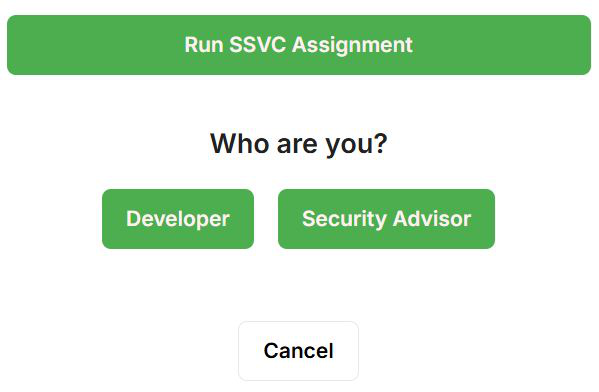
\includegraphics[scale=0.6]{resources/SSVC_Input.png}
    \caption{Interactive Decision Tree Interface: Initial role selection.}
    \label{fig:ssvc-tree-interface}
\end{figure}

Each response is processed to build a comprehensive recommended action plan, consisting of advisories such as \enquote{Apply patch immediately} when a vendor patch is available. Below is a code snippet demonstrating the logic for handling decisions within the tree structure and compiling the responses into a final recommendation. For example, one decision involves checking whether a vendor patch is available. Based on this, subsequent steps, such as applying the patch or exploring alternative mitigations, are determined.

\paragraph{Pseudocode for Decision Handling}
The following pseudocode demonstrates how decisions are processed to generate a recommendation:

\begin{verbatim}
// Generate recommendation based on patch availability
function generateRecommendation(data):
    recParts = []  // Collect recommendation parts

    if data.getPatchAvailableDev() == "yes":
        recParts.push("Vendor patch is available. Apply immediately.")
    else:
        recParts.push("No vendor patch found. Develop a custom fix.")

    return "Developer: " + recParts.join(" ")
\end{verbatim}

\paragraph{Final Recommendation}
After collecting all partial recommendations, the final message is composed and delivered (see example figure~\ref{fig:ssvc-recommendation}):

\begin{verbatim}
// Compile and deliver final recommendation
finalMessage = "Developer: " + recParts.join(" ")
setSuccessMessage(finalMessage)
onComplete(finalMessage)
\end{verbatim}

\begin{figure}[H]
    \centering
    
\includegraphics[width=0.8\linewidth]{resources/SSVC_Recommandation.png}
    \caption{Example of a final recommendation message delivered to a developer.}
    \label{fig:ssvc-recommendation}
\end{figure}

\subsection{Score Details Button}
A \textit{Show Score Details} popup (as described in section \ref{subsec:ui-explaining-score}) allows users to see the \ac{CVE}-ID, the \ac{CVSS} score and vector, the \ac{EPSS} score, the computed severity, and a textual explanation as described in section \ref{subsec:ui-explaining-score}. This is done through:

\begin{itemize}
  \item \textbf{Button Trigger:} A button in the \enquote{Vulnerability Details} view opens a modal dialog.
  \item \textbf{Dialog Contents:} The modal includes fields for the \ac{CVE} ID, \ac{CVSS} V3.1 base score, vector string, \ac{EPSS} metric, and the final severity. If any fields are missing, placeholders (e.g., \texttt{N/A}) or a note about further actions that can be taken are shown.
  \item \textbf{Hover Tooltips for Vectors:} Displays hover-based tooltips for each \ac{CVSS} vector attribute. When the user places the cursor over a specific field (e.g., \enquote{Attack Vector} or \enquote{Attack Complexity}), a concise explanation appears to clarify its impact on the vulnerability assessment.
  \item \textbf{Direct Link to the \ac{CVSS} Calculator:} Provides a direct link to the official \ac{CVSS} calculator.\footnote{\url{https://nvd.nist.gov/vuln-metrics/cvss/v3-calculator}} This link is automatically populated with the relevant vector data, allowing users to quickly review the existing metrics and explore different scoring scenarios.
\end{itemize}

This functionality is illustrated in figure~\ref{fig:score-details}, which shows an example of the \textit{Score Details} popup.

\begin{figure}[H]
    \centering
    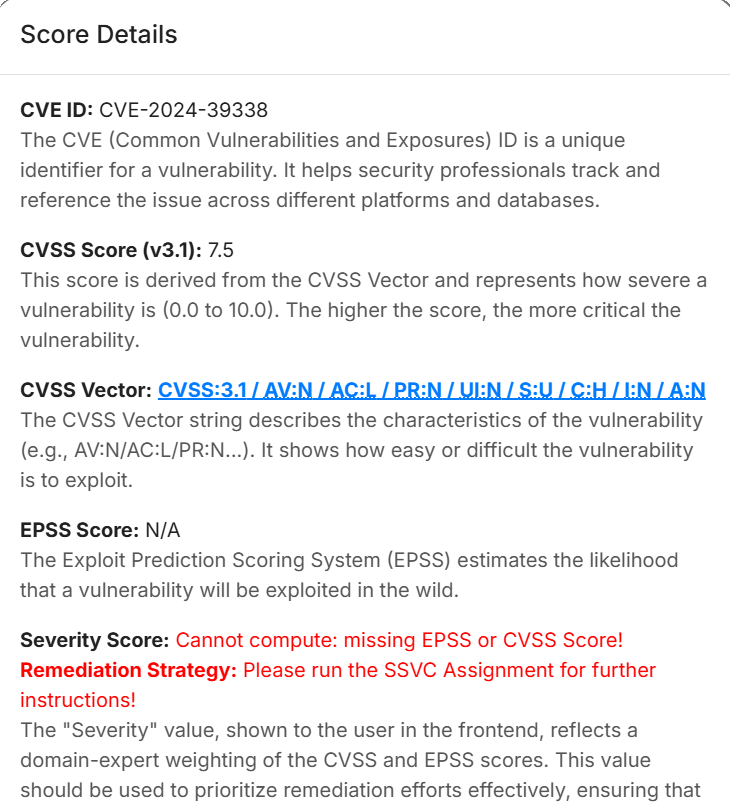
\includegraphics[scale=0.45, trim=2mm 2mm 2mm 2mm, clip]{resources/Score_Details_Button.PNG}
    \caption{Example of the \textit{Show Score Details} popup showing diverse data their explanation, and recommendations.}
    \label{fig:score-details}
\end{figure}

\section{Ranking and Prioritization Of All Vulnerabilities}
\label{sec:ranking-implementation}

This section describes the implementation of the model introduced in section~\ref{sec:rank-order-vulnerabilities}, focusing on how vulnerabilities are ranked and prioritized based on their severity.

\subsection{Descending Sort of Precalculated Severity Scores and Handling Missing Data}
The implementation takes the precalculated severity scores, which include contributions from \ac{CVSS} and \ac{EPSS}, and sorts them in descending order. This ensures that vulnerabilities with the highest severity scores are prioritized, while those with missing data are given placeholder scores for immediate attention.

For vulnerabilities with missing essential data, a placeholder score of \textbf{10.1} is assigned. This score exceeds the maximum valid severity of 10.0, ensuring these entries are sorted to the top of the list. In the user interface, such entries are highlighted with a pink \textbf{“UNKNOWN”} label, prompting users to investigate and resolve the missing information.

An example of the sorted list, as displayed in the user interface, is shown in figure~\ref{fig:rank-order-example}, where placeholder scores for missing data are indicated by a pink \enquote{UNKNOWN} label.

\begin{figure}[H]
    \centering
    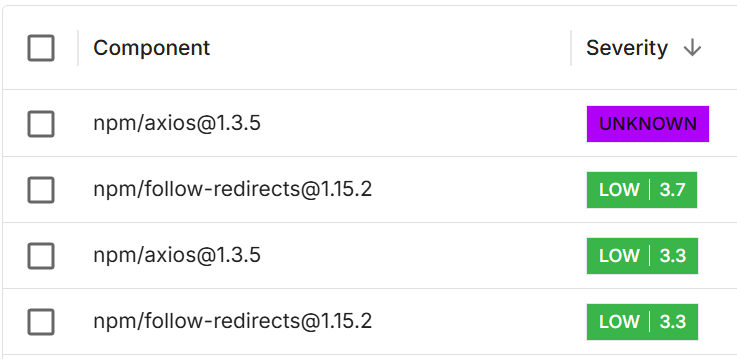
\includegraphics[scale=0.7]{resources/Rank-Order.PNG}
    \caption{Example of a sorted list of vulnerabilities in descending order of severity.}
    \label{fig:rank-order-example}
\end{figure}

\section{Conclusion}
\label{sec:implementation-conclusion}

The implementation details presented in this chapter show how the multi-dimensional vulnerability classification and remediation framework (see chapter~\ref{chapter:multidimensional-vulnerability-classification}) and the proposed system design (see chapter~\ref{chapter:design}) have been realized in a fully functional solution that integrates both backend and frontend components. Critical elements, such as caching and scheduled refresh (see section~\ref{subsec:caching-repository}), ensure that vulnerability data remains reliable, and continuously up-to-date, while minimizing external lookups.

The system interaction workflow (see section~\ref{subsec:system-interaction}) highlights how local \ac{OSV} data is leveraged, triggering external lookups for \ac{CVSS} and \ac{EPSS} only when strictly necessary. Building on these processes, the \ac{SSVC} endpoint (see section~\ref{par:ssvc-recommendation-endpoint}) and role-specific frontend logic (see section~\ref{sec:frontend-components}) enable targeted remediation recommendations for different user roles.

Moreover, combining \ac{CVSS} and \ac{EPSS} metrics captures both technical severity and exploitability factors in accordance with the multi-dimensional model. Finally, the ranking and visualization (see section~\ref{sec:ranking-implementation}) allow for effective prioritization of vulnerabilities, with any missing data explicitly flagged via a placeholder severity score (e.g., \textbf{10.1}). Taken together, these components form a cohesive, user-focused system that significantly streamlines vulnerability management and remediation activities, fulfilling the objectives outlined in earlier chapters.


